\documentclass[letterpaper,titlepage]{article}
\usepackage[margin=0.9in]{geometry}
\usepackage{
    tocloft,
    graphicx,
    hyperref,
    float
}
\usepackage[table,xcdraw]{xcolor}
\usepackage[backend=biber]{biblatex}

% Single space after period
\frenchspacing

% Color links blue
\hypersetup{
    colorlinks,
    urlcolor=blue,
    linktoc=section,
    linkcolor=blue
}

% Add dots to TOC
\renewcommand\cftsecleader{\cftdotfill{\cftdotsep}}

% Set graphics path
\graphicspath{{./Figures}}

% Add bibliography
\addbibresource{References.bib}
% Print references without being cited in-text
\nocite{*}

% Title page
\title{Predicting the Next Defensive Player of the Year in the NBA}
\author{
    Joshua Samuel \\ \href{mailto:jsamuel41@tamu.edu}{jsamuel41@tamu.edu}
    \and
    Alex LeGresley \\ \href{mailto:alexlegresley@tamu.edu}{alexlegresley@tamu.edu}
}
\date{Texas A\&M University}


\begin{document}

    \maketitle
    \pagenumbering{gobble}
    \tableofcontents
    \clearpage
    \pagenumbering{arabic}


    \section{Importance of Study}
    We seek to predict the winner of this year's NBA's Defensive Player of the Year Award, in addition to identifying other players who will be in contention for the award and how they will stack up. The Defensive Player of the Year (DPOY) award is one of the most coveted awards given for the performance of NBA players during the regular season, second only to the overall Most Valuable Player of the Year Award. With betting continuing to become more and more prevalent in sports, the amount of money won and lost regarding regular season awards continues to increase dramatically. Furthermore, player contracts often contain lucrative incentives for winning regular season awards, nevertheless the intangible boost to one's legacy and status in the game. Thus, statistical prediction of the DPOY award is of potential importance to a variety of parties.

    
    \section{Exploratory Data Analysis}

    \subsection{Description of Dataset}
    The dataset used in this analysis was aggregated from various collections provided by Basketball Reference. The data was obtained in CSV and Excel format. It comprises of four primary datasets spanning the NBA seasons from 1982-1983 to 2022-2023. The first dataset encompasses standard statistics (such as blocks, steals, etc.) of all active players who participated in at least one game during this period. The second dataset consists of advanced metrics (including box plus/minus, win shares, etc.) of the same players. The third dataset, covering the same time frame, lists every player who received at least one vote for the Defensive Player of the Year award in each respective season. The fourth and final dataset adds the respective team standings position for every player in the dataset.

    \subsection{Data Cleaning}
    Duplicates were removed from each dataset, specifically instances where a player switched teams within a season. Instead of retaining separate observations for each team, the statistics for such players were aggregated for the entire season. The team rank associated with players who played for multiple teams during a season was taken to be the average of the teams ranks they played for weighted by the number of minutes played for each team. Ultimately, each row of the dataset was a unique combination of player and season. A few columns provided in the Basketball-Reference dataset did not have meaningful associated names and thus were dropped since they could not be confidently regarded as a known metric. This led to a total of 49 meaningful covariance and one response variable.
    
    While the details of the statistical models will be covered in detail later, data setup was necessary to be congruent with their limitations. All but one of the covariates was quantitative, with the player position being multi-class categorical. The XGBoost implementation provides built-in support for handling categorical variables, however the Scikit-Learn implementation of linear models does not. Dummy variables for player position were created for use with the linear models. Furthermore, many of the quantitative covariates had missing values. The XGBoost implementation also provides built-in support for handling missing values, however the Scikit-Learn linear models implementation does not. Median imputation was used to fill the missing values for use with the linear models. We chose median imputation due to the median being more robust to skewness, as we anticipated some of the covariates would be skewed.

    \subsection{Summary Statistics}
    The distribution of the share of Defensive Player of the Year Award votes is highly right-skewed, with a vast majority of players having a vote share of zero. There is nearly a 30:1 ratio of players who did not receive a DPOY award vote to those who received at least one vote. This important characteristic of the data is accounted for in our methodology.


    \section{Methodology}
    
    To address the significant imbalanced nature of the voting for the DPOY award due to very few players receiving any votes, we will employ a two stage process.

    \subsection{Stage 1}
    The first stage model aims to classify whether a player is likely to receive any votes for the Defensive Player of the Year award. We will build the stage 1 model first with XGBoost, then compare the performance with a simpler logistic regression model. For this model, we will transform the response variable, which is the DPOY vote share for each player in each season, to a binary outcome: 1 if they received any share, that is their vote share is non-zero, and zero otherwise. The classes will be very unbalanced, with many zeros and a few ones. We will balance the classes in the statistical model training process by adjusting the class weights such that the observations of players who received a vote will be weighted higher. Specifically, the class weights will correspond to a 30:1 ratio as found during the exploratory data analysis process. 
    
    Model performance will be evaluated using the metric area under the precision recall curve (AUCPR). This metric is advantageous in scenarios with significant class imbalance since it will penalize false negatives. This is necessary because a model that only predicts zero would have a high accuracy but ultimately not be useful. We will use cross-validation when evaluating potential models, as it provides a statistically more reliable estimation of the performance than a single train/test split. Specifically, we will use stratified k-fold cross-validation. Stratification is necessary due to the class imbalance, as it helps ensure an approximately equal representation of classes in each group compared to standard k-fold cross-validation. Furthermore, the model will output probabilities of belonging to the positive class, that is receiving any vote share, and it is up to us to determine whether the probability is high enough to expect the player to receive any vote share. 
    
    We will tune this probability threshold using the F1 score metric, which is also a robust metric in cases of class imbalance. Ultimately, the stage 1 model will act as a filter, removing those who are unlikely to receive any votes. We can then take those who we expect to receive at least one vote and inspect on a more granular level to determine the specific amount of vote share.

    \subsection{Stage 2}
    The second stage model predicts the amount of share in the Defensive Player of the Year Award for players classified in the previous model as projected to receive a share. We will build the stage 2 model with XGBoost, then compare the performance with a simpler linear regression model. The player predicted to have the highest share in a given season is expected to win the award.
    
    We will work with the response variable as a continuous quantitative variable and while utilizing the same covariates as the first model. Model performance will be evaluated using the metrics root mean squared error (RMSE) and \(R^2\). RMSE is a robust standardized metric that indicates how well the model is able to predict the response variable, while \(R^2\) indicates how well the covariates explain the variation in the response. Furthermore, we will use cross-validation when evaluating potential models. Specifically, k-fold cross-validation since the response is quantitative.


    \section{Stage 1 Model}

    XGBoost classifier models were fit. The dataset consists of 17900 observations (all players appearing in at least one game from the 1982-1983 to 2022-2023 seasons) with 49 covariates (48 quantitative, 1 categorical) and 1 binary response. The class weights were adjusted to account for the imbalance and stratified cross-validation employed with evaluation by AUCPR. The built-in implementation handling of categorical predictors and missing observations was also used.

    \subsection{Initial Results}
    We initially fit the model with default hyperparameters. This yielded an average AUCPR from cross-validation of 0.478 and an average F1 score from cross-validation of 0.469. These values suggest that the model is similar to a coin flip in terms of determining whether a player is likely to have received at least one DPOY vote, and thus there is much room for improvement in the predictive performance of the model.

    \subsection{Tuning}
    We turned to tuning the hyperparameters of the model as a source of potential improvement. We identified the XGBoost hyperparameters learning rate, maximum depth of trees, and number of estimators as being most likely to result in significantly enhanced predictive performance. We chose a randomized search technique due to the balance between computational efficiency and ability to search a wide space of potential values for the hyperparameters. Specifically, randomized search helps find optimal hyperparameter values by randomly sampling with replacement from a given statistical distribution of hyperparameter values. This randomized search process was ran with 75 iterations of stratified 5-fold cross-validation. The hyperparameters leading to the model with the maximum AUCPR were considered optimal.

    \subsection{Post-Tuned Results}
    The average AUCPR from cross-validation for our best model was 0.609 with the best parameters being 0.153 for the learning rate, 11 for the max tree depth, and 162 for the number of estimators. We next tuned the probability decision threshold for considering a player to receive at least one DPOY vote. Stratified 5-fold cross-validation was used to test thresholds in increments of 0.05 with evaluation by F1 score. The average best threshold from cross-validation was 0.35 with a corresponding average F1 score from cross-validation of 0.581.

    The feature importance chart \autoref{fig:Stage1FeatImp} shows the relative importance of each feature in the model. Features with higher importance have more influence on the model's predictions, while those with lower importance have less. It is not surprising to see defensive metrics such as Personal Fouls (PF), Defensive Box Plus Minus (DBPM), and Defensive Win Share (DWS) near the top in terms of influence. However, it is surprising to see Steal \% (STL\%) with the least influence, as this is a commonly cited defensive metric.

    \begin{figure}[H]
        \centering
        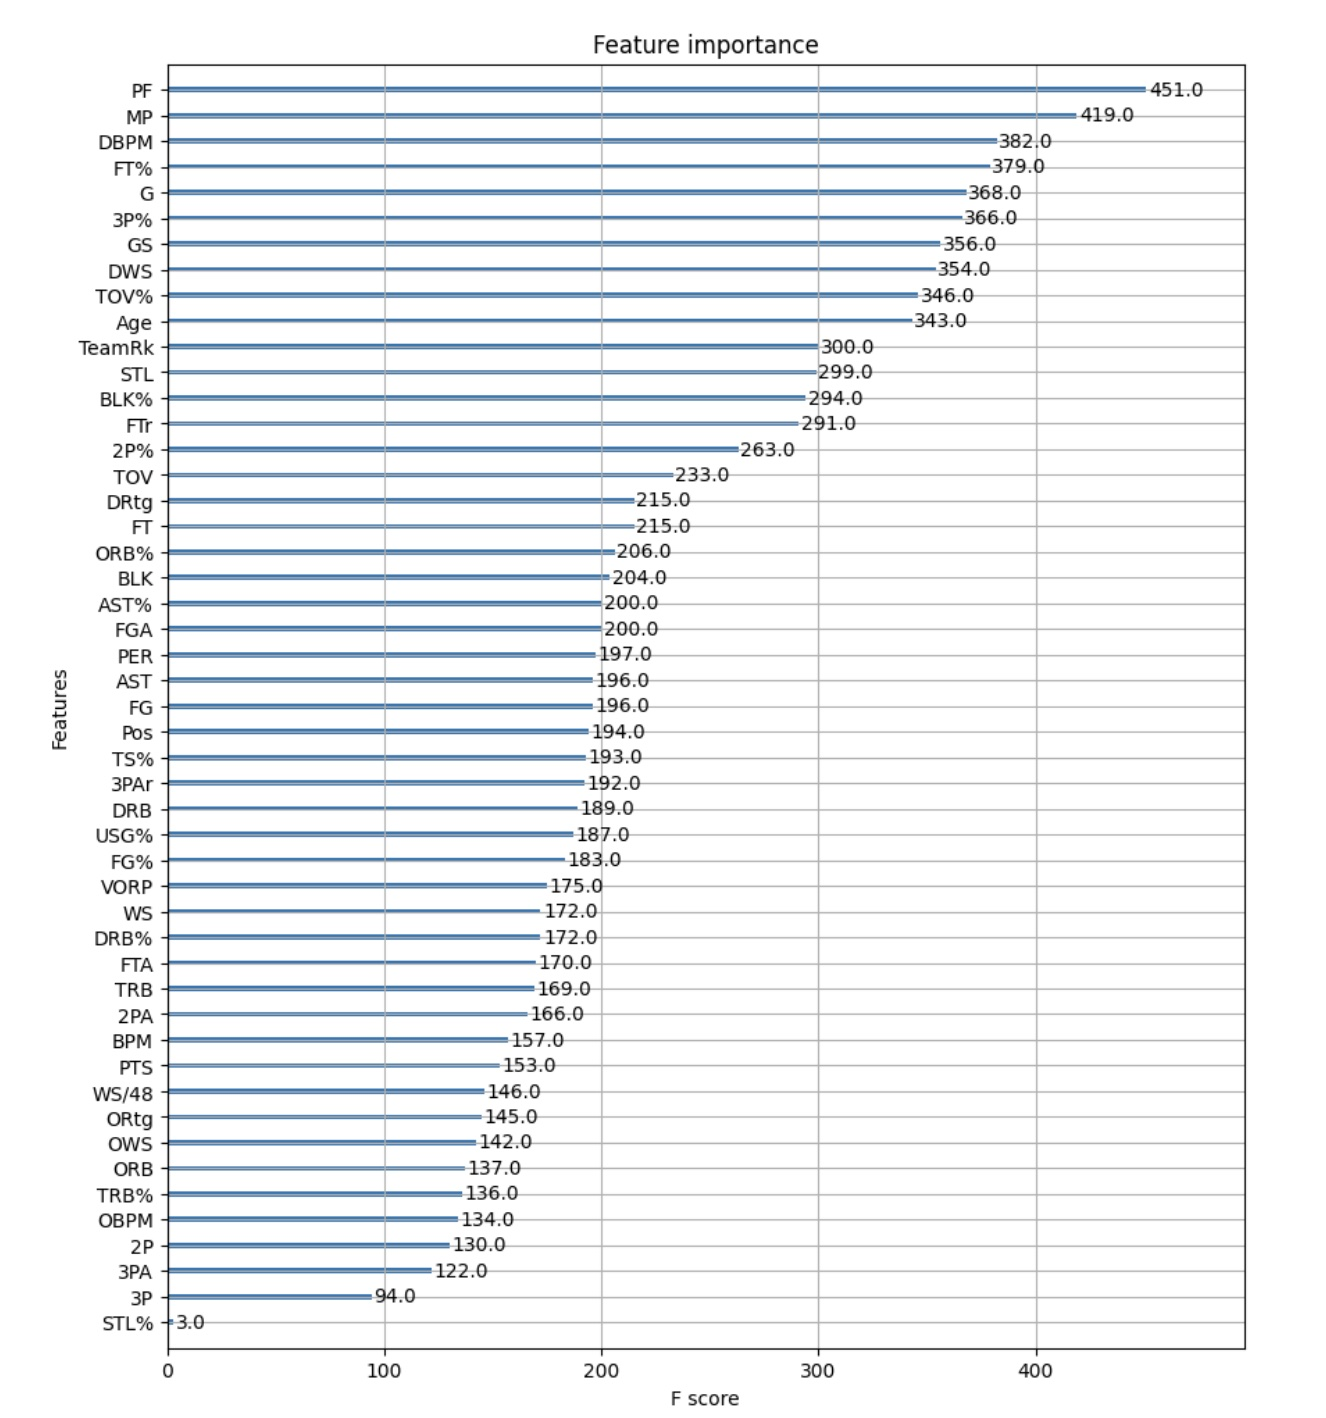
\includegraphics[scale=0.27]{Stage_1_Feature_Importance.jpg}
        \caption{Stage 1 feature importance for tuned XGBoost classifier model}
        \label{fig:Stage1FeatImp}
    \end{figure}    

    \subsection{Logistic Model Comparison}
    To investigate whether a complex model such as XGBoost is necessary, we compared the performance to a simpler logistic regression model. Class weights were adjusted to account for the imbalance. Dummy variables were created for the categorical Position covariate and missing data for quantitative covariates was imputed using the median. Random search with 75 iterations of stratified 5-fold cross-validation was used to tune the C hyperparameter, which controls the aggressiveness of the regularization process. The optimal model was that which maximized AUCPR.

    The best logistic regression model had an average AUCPR from cross-validation of 0.496. The probability decision threshold was optimized by employing stratified 5-fold cross-validation to test thresholds in increments of 0.05 with evaluation by F1 score. The maximum average F1 score from cross-validation was 0.524 achieved at a threshold of 0.90.

    The AUCPR and F1 score for the logistic regression model was slightly lower than those of the XGBoost model. Thus, we conclude that the XGBoost model has slightly better predictive performance.

    
    \section{Stage 2 Model}

    XGBoost regressor models were fit. The dataset consists of 575 observations (players receiving any vote share from the 1982-1983 to 2022-2023 seasons) with the same 49 covariates (48 quantitative, 1 categorical) as the stage 1 model and 1 quantitative response. K-fold cross-validation and evaluation by RMSE was used to select the best model. The built-in implementation handling of categorical predictors and missing observations was also used.

    \subsection{Tuning}
    We tuned the same XGBoost hyperparameters as in stage 1, those being learning rate, max tree depth, and number of estimators. Randomized search was used with 75 iterations of 5-fold cross-validation with evaluation by -RMSE. The use of -RMSE rather than RMSE is an implementation detail consequence of the Sckikit-Learn Unified Scoring API. The interpretation is the same, that is a score closer to zero represents less prediction error and is desirable. The model that minimized -RMSE was considered optimal.

    \subsection{Post-Tuned Results}
    The average -RMSE from cross-Validation for our best model was -0.153 with the best parameters being 0.097 for the learning rate, 3 for the max tree depth, and 94 for the number of estimators. Furthermore, the average \(R^2\) from cross-validation was 0.292. This means that our model explains only about 29.2\% of the variability in DPOY vote share, and thus there is definitely room for improvement.

    The feature importance chart \autoref{fig:Stage2FeatImp} shows the relative importance of each feature in the XGBoost model. Advanced defensive metrics such as Defensive Win Shares (DWS) and Defensive Box Plus Minus (DBPM) were considered the two most important features which is not surprising. However, Blocks (BLK) and Defensive Rebounding Percentage (DRB\%) being low in terms of importance is surprising given that they are considered by many to be important defensive statistics. Field Goal Percentage (FG\%) being ranked 7th in importance illustrates how the efficiency of a player on the offensive end still plays a factor in whether they win the award. 

    \begin{figure}[H]
        \centering
        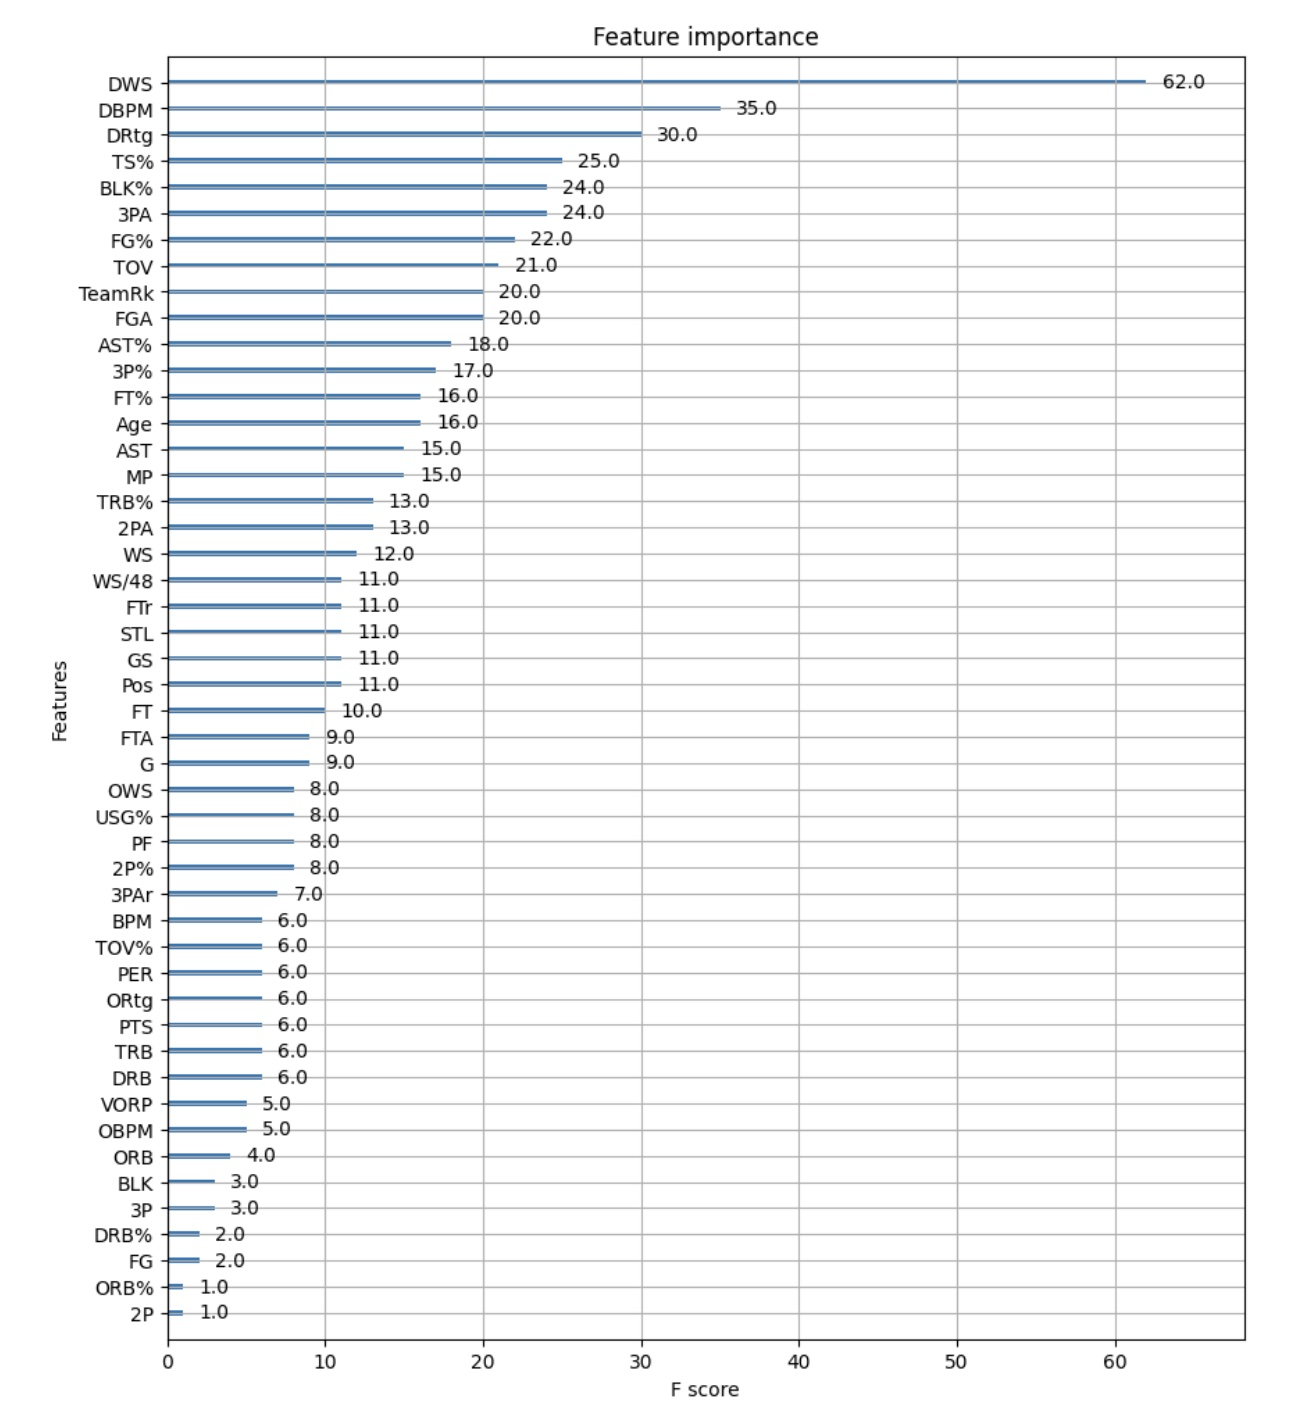
\includegraphics[scale=0.27]{Stage_2_Feature_Importance.jpg}
        \caption{Stage 2 feature importance for XGBoost regressor model}
        \label{fig:Stage2FeatImp}
    \end{figure}

   \subsection{Linear Model Comparison}
    To investigate whether a complex model such as XGBoost is again necessary, we compared the performance to a simpler linear regression model. Dummy variables were created for the categorical Position covariate and missing data for quantitative covariates was imputed using the median. Reverse Feature Elimination (RFE) was used to identify the optimal number of predictors to include in the model. This was run with 75 iterations of 5-fold cross-validation and the best model identified based on minimizing -RMSE.

    The best linear regression model had an average -RMSE from cross-validation of -0.167 and an average \(R^2\) from cross-validation of 0.200. Thus, the linear regression model has slightly higher prediction error and explains slightly less of the variability in vote share compared to the XGBoost regressor model.


    \section{Current Season Results}

    In line with our goal, we tested the stage 1 and stage 2 XGBoost models and the stage 1 and stage 2 linear models with the current NBA season data to predict this year's Defensive Player of the Year. The current season has concluded so all data is available, however the award has not yet been given out. The predictions using the stage 1 and stage 2 XGBoost models are shown in \autoref{Tab:XGRes}, the stage 1 and stage 2 linear models in \autoref{Tab:LMRes}, and the current Vegas betting odds from the DraftKings Sportsbook as of 4/17/2024 in \autoref{Tab:Vegas}.

    Our XGBoost process performed quite well as the top 4 DPOY candidates according to Vegas are accounted for in the top 8 for our preferred process. Our XGBoost's top 2 candidates are the same as Vegas however the order is different. Our linear model process had a few of the same projected candidates as our XGBoost process. However, there are two very significant outliers at the top of the linear process's ranking, as background knowledge of the NBA season reinforces that Markquis Nowell and Hamidou Diallo are in reality nowhere close to being in consideration for the award. The two players currently play in the development league (G League) of their respective teams and will occasionally be called up to play for the actual NBA team.

    \begin{table}[H]
        \centering
        \caption{XGBoost predicted DPOY vote share}
        \label{Tab:XGRes}
        \begin{tabular}{c|c|c}
            \textbf{Place} & \textbf{Player}         & \textbf{Vote Share} \\ \hline
            \rowcolor[HTML]{EFEFEF}
            1              & Victor Wembanyama       & 0.345               \\ 
            2              & Rudy Gobert             & 0.283               \\
            \rowcolor[HTML]{EFEFEF}
            3              & Chet Holmgren           & 0.185               \\ 
            4              & Kristaps Porzingis      & 0.182               \\
            \rowcolor[HTML]{EFEFEF} 
            5              & Anthony Davis           & 0.144               \\ 
            6              & Giannis Antetokounmpo   & 0.137               \\
            \rowcolor[HTML]{EFEFEF}
            7              & Shai Gilgeous-Alexander & 0.135               \\
            8              & Bam Adebayo             & 0.062               \\
            \rowcolor[HTML]{EFEFEF} 
            9              & Nic Claxton             & 0.008              
        \end{tabular}
    \end{table}

    \begin{table}[H]
        \centering
        \caption{Linear model predicted DPOY vote share}
        \label{Tab:LMRes}
        \begin{tabular}{c|c|c}
            \textbf{Place} & \textbf{Player}          & \textbf{Vote Share} \\ \hline
            \rowcolor[HTML]{EFEFEF} 
            1              & Markquis Nowell          & 0.587               \\
            2              & Hamidou Diallo           & 0.351               \\
            \rowcolor[HTML]{EFEFEF} 
            3              & Rudy Gobert              & 0.321               \\
            4              & Chet Holmgren            & 0.152               \\
            \rowcolor[HTML]{EFEFEF} 
            5              & Victor Wembanyama        & 0.147               \\
            6              & Anthony Davis            & 0.143               \\
            \rowcolor[HTML]{EFEFEF} 
            7              & Shai Gilgeous-Alexander  & 0.142               \\
            8              & Isaiah Hartenstein       & 0.131               \\
            \rowcolor[HTML]{EFEFEF} 
            9              & Josh Hart                & 0.130               \\
            10             & Nikola Jokic             & 0.124               \\
            \rowcolor[HTML]{EFEFEF} 
            11             & Derrick White            & 0.116               \\
            12             & Herbert Jones            & 0.110               \\
            \rowcolor[HTML]{EFEFEF} 
            13             & Shaquille Harrison       & 0.108               \\
            14             & Giannis Antetokounmpo    & 0.089               \\
            \rowcolor[HTML]{EFEFEF} 
            15             & Brook Lopez              & 0.080               \\
            16             & Kentavious Caldwell-Pope & 0.073               \\
            \rowcolor[HTML]{EFEFEF} 
            17             & Jrue Holliday            & 0.069              
        \end{tabular}
    \end{table}

    \begin{table}[H]
        \centering
        \caption{DraftKings Sportsbook DPOY odds as of 4/17/2024}
        \label{Tab:Vegas}
        \begin{tabular}{c|c}
            \textbf{Player}   & \textbf{Odds} \\ \hline
            \rowcolor[HTML]{EFEFEF} 
            Rudy Gobert       & -3,000        \\
            Victor Wembanyama & +1,000        \\
            \rowcolor[HTML]{EFEFEF} 
            Bam Adebayo       & +20,000       \\
            Anthony Davis     & +20,000       \\
            \rowcolor[HTML]{EFEFEF} 
            Jarret Allen      & +20,000       \\
            Derrick White     & +20,000      
        \end{tabular}
    \end{table}


    \section{Final Conclusions \& Future Modifications}
    Our two-stage XGBoost model process predicts with reasonable accuracy which players will be near the top of the DPOY award voting based off data from a given regular season. We have also been able to identify which metrics contribute most (and least) significantly in predicting how much of a share in DPOY votes a player will receive. We have seen how our preferred tuned XGBoost models outperform our more elementary linear models. In the future, we would consider taking into account the years of NBA experience a player has, since typically the DPOY award is not given to rookies. While we did have an "age" predictor, an additional "years of experience" predictor would be helpful given players enter the league at various ages.

    A limitation of our model is that the final predictions are not restricted such that the vote shares sum to one. This is an issue if the specific vote share itself if highly desired to be accurate. In our case, we cared more about the relative rankings of the players in terms of the order they will finish in the voting. In the future, we would like to refine the model to address this limitation and thus produce more realistic vote shares.


    \section{Code \& Data}
    The data files and a Python notebook containing the code used to produce all of the analyses can be obtained from \url{https://github.com/alexlegresley/STAT482-Capstone}.


    \printbibliography[heading=bibnumbered]
    
\end{document}